\section{Performance Evaluation}
%In this section, we evaluate the performance of \sol~and
%compare it with Swarmkit management tool from Docker.

\begin{figure*}[ht]
%\hspace*{0.8in}
   \centering
%\vspace{-0.1in}
      \begin{subfigure}[t]{0.32\linewidth}
\centering
      \includegraphics[width=\linewidth]{25memcpu1}
      \vspace{-0.15in}
      \caption{Worker 1 (Spread, 100)}
      \label{fig:25worker1}
      \end{subfigure} %
      ~%%%%%%%%%%%%%%%%%%%%%%%%%%%%%%%%
      \begin{subfigure}[t]{0.32\linewidth}
\centering
      \includegraphics[width=\linewidth]{25memcpu2}
      \vspace{-0.15in}
      \caption{Worker 2 (Spread, 100)}
      \label{fig:25worker2}
      \end{subfigure} %
      ~
      \begin{subfigure}[t]{0.32\linewidth}
\centering
      \includegraphics[width=\linewidth]{25memcpu3}
      \vspace{-0.15in}
      \caption{Worker 3 (Spread, 100)}
      \label{fig:25worker3}
      \end{subfigure} %
      
   \centering
%\vspace{-0.1in}
      \begin{subfigure}[t]{0.32\linewidth}
\centering
      \includegraphics[width=\linewidth]{25memcpu1g}
      \vspace{-0.15in}
      \caption{Worker 1 (\sol, 100)}
      \label{fig:25worker1g}
      \end{subfigure} %
      ~%%%%%%%%%%%%%%%%%%%%%%%%%%%%%%%%
      \begin{subfigure}[t]{0.32\linewidth}
\centering
      \includegraphics[width=\linewidth]{25memcpu2g}
      \vspace{-0.15in}
      \caption{Worker 2 (\sol, 100)}
      \label{fig:25worker2g}
      \end{subfigure} %
      ~
      \begin{subfigure}[t]{0.32\linewidth}
\centering
      \includegraphics[width=\linewidth]{25memcpu3g}
      \vspace{-0.15in}
      \caption{Worker 3 (\sol, 100)}
      \label{fig:25worker3g}
      \end{subfigure} %
      
\caption{Memory and CPU resources usage comparison between Spread and \sol~placement scheme (100 containers)}
\label{fig:noworkload25}
\end{figure*}

\subsection{Implementation, Testbed and Workloads}
We implement our new container placement 
scheme, \sol, on Docker Community Edition (CE) v17. 
As described in Section~\ref{sys}, the major modules in \sol~are integrated into the existing
Docker Swarmkit framework. 

To evaluate \sol, we build a heterogeneous cluster on Alibaba Cloud~\cite{aliyun}, which supports multiple types of computing nodes.
Specifically, we use three different types of instances, small (1 CPU core and 4G memory), medium (4 CPU cores and 8G memory)
and large (8 CPU cores and 16G memory).
In the small-scale testing, we setup a cluster with 3 nodes, one of each type, and configure it with 1 manager and 3 worker (1 of the 3 physical nodes 
hosts both manager and worker). In experiments on scalability, we configure the cluster with 1 manger and 9 workers that consist 3 instances of each type. 

%We consider two different categories, workloads for the cluster and for services provided by containers.
The main objective of \sol~is to understand resource demands of services and place them on appropriate worker nodes.
As we discussed in Section~\ref{understand}, characteristics of services are varied. 
Therefore, workloads for the cluster are images of various services. In the evaluation,
we select 18 different images in 4 types from Docker Hub~\cite{dockerhub} to build our image pool. 
{\bf Database Services}:  MongoDB, MySQL, Postgres, Cassandra, RethinkDB.
{\bf Storage/Caching Services}:  Registry, Memcached.
{\bf Web Services}: Tomcat, Httpd, Redis, HAProxy, Jetty, Nginx, GlassFish.
{\bf Message Services}: RabbitMQ, Apache ZooKeeper, ActiveMQ, Ghost.




\subsection{Evaluation Results}
\subsubsection{Idle containers}
In this subsection, we present the result of a cluster with idle containers.
If a container is in a running state but does not serve any clients, we call it a idle container.
Idle container is an important concept since every node, right after initialization will act as an idle container.
Understanding the resource demands of an idle container will help us select its host.
In these experiments, we first randomly choose 14 images form the pool, and each image will be used to initiate 10
containers. Therefore, there are 140 containers in the cluster. 
Those containers are started one by one with 5 seconds interval. 
This is because previous containers will result in  different available resources on worker nodes, which we can utilize 
to test \sol.

Fig~\ref{fig:noworkload25} illustrates a comparison of memory and CPU usages between Spread, 
a Swarmkit default placement scheme, with \sol. As we can see from the subfigures, most of the CPU usage happens from 0 to 500s.
This is caused by submission pattern that used to initiate containers. The percentage grows continuously from 0 to 500s since
we have 100 containers and the submission interval is 5 seconds. While in both systems, the usage of CPU stays at a low level on average. 
However, the memory usage keeps increasing along with the number of containers on each worker. 
Due to the idle container setting, the utilization of memory is stable after 500s (all the containers 
have successfully initiated). There are some jitters on the curve of CPU, because 
some supporting programs, such as the Docker engine and service daemon, are running on the same worker and, of course, they are consuming resources. 
Comparing the memory usage rates after 500s, \sol~significantly reduces rate on worker 1, from 80.5\% to 46.7\%. 
On worker 2, Spread and \sol~achieve similar performance on memory, 39.1\% verse 40.6\%.
On worker 3, Spread results in 23.6\% and \sol~consumes 33.3\%. The \sol~outperforms Spread by considering the heterogeneity in the cluster and 
various resource demands of services. When a task arrives at the system, it selects a worker based on the service demands and current available resources.
Fig~\ref{fig:num} shows the number of containers on workers. For Swarmkit with Spread, it uses a bin-pack strategy and tries to equally distribute
the containers to every worker, which results in 34, 33, 33 containers for worker 1, 2, 3. While in \sol, worker 3 has more power than others and hosts more 
containers than worker 1, which has limited resource.
\begin{comment}
\begin{figure}[h]
\centering
\begin{minipage}[t]{width=0.24\linewidth}
\centering
\includegraphics[width=\linewidth]{25containernum}
\caption{Number of containers on each worker}
\label{fig:num} 
\end{minipage}
~
\begin{minipage}[t]{width=0.24\linewidth}
\centering
\includegraphics[width=\linewidth]{25net}
\caption{Network usage comparison on worker 3}
\label{fig:25net} 
\end{minipage}
\end{figure}
\end{comment}


\begin{figure}[ht]
%\hspace*{0.8in}
   \centering
%\vspace{-0.1in}
      \begin{minipage}[t]{0.48\linewidth}
\centering
      \includegraphics[width=\linewidth]{25containernum}
      \caption{Number of containers on each worker}
      \label{fig:num} 
      \end{minipage} %
      %%%%%%%%%%%%%%%%%%%%%%%%%%%%%%%%
      \begin{minipage}[t]{0.48\linewidth}
\centering
      \includegraphics[width=\linewidth]{25net}
      \caption{Network consumption comparison on worker 3}
      \label{fig:25net}
      \end{minipage} %
%\caption{Resource demonds under different workloads on four services, MySQL, Tomcat, YUM, PI.}
\end{figure}



While \sol~achieves better performance, it introduces more data transfers between managers and workers through heartbeat messages.
Fig~\ref{fig:25net} plots the network consumption of Swarmkit and \sol~ on worker 3, which hosts both a manager and a worker. 
As expected, \sol~ consumes more bandwidth than Swarmkit due to the enhanced heartbeat messages includes more statistical information resource
usages of containers. Considering the distributed architecture, the system can have multiple managers and each of them in charge of controllable
number of workers, the increase of bandwidth consumption that brought by \sol~ is reasonable.


\begin{figure*}[ht]
%\hspace*{0.8in}
   \centering
%\vspace{-0.1in}
      \begin{subfigure}[t]{0.32\linewidth}
\centering
      \includegraphics[width=\linewidth]{memcpu1}
      \vspace{-0.15in}
      \caption{Worker 1 (Spread, 140)}
      \label{fig:worker1}
      \end{subfigure} %
      ~%%%%%%%%%%%%%%%%%%%%%%%%%%%%%%%%
      \begin{subfigure}[t]{0.32\linewidth}
\centering
      \includegraphics[width=\linewidth]{memcpu2}
      \vspace{-0.15in}
      \caption{Worker 2 (Spread, 140)}
      \label{fig:worker2}
      \end{subfigure} %
      ~
      \begin{subfigure}[t]{0.32\linewidth}
\centering
      \includegraphics[width=\linewidth]{memcpu3}
      \vspace{-0.15in}
      \caption{Worker 3 (Spread, 140)}
      \label{fig:worker3}
      \end{subfigure} %
      
   \centering
%\vspace{-0.1in}
      \begin{subfigure}[t]{0.32\linewidth}
\centering
      \includegraphics[width=\linewidth]{memcpu1g}
      \vspace{-0.15in}
      \caption{Worker 1 (\sol, 140)}
      \label{fig:worker1g}
      \end{subfigure} %
      ~%%%%%%%%%%%%%%%%%%%%%%%%%%%%%%%%
      \begin{subfigure}[t]{0.32\linewidth}
\centering
      \includegraphics[width=\linewidth]{memcpu2g}
      \vspace{-0.15in}
      \caption{Worker 2 (\sol, 140)}
      \label{fig:worker2g}
      \end{subfigure} %
      ~
      \begin{subfigure}[t]{0.32\linewidth}
\centering
      \includegraphics[width=\linewidth]{memcpu3g}
      \vspace{-0.15in}
      \caption{Worker 3 (\sol, 140)}
      \label{fig:worker3g}
      \end{subfigure} %
      
\caption{Memory and CPU resources usage comparison between Spread and \sol~placement scheme (140 containers)}
\label{fig:noworkload35}
\end{figure*}


Next, we conduct the same experiments with 40\% more containers to test the scalability of \sol.
Fig~\ref{fig:noworkload35} plots the system performance with 140 Docker containers. Comparing the figures, the first impression is that
on Fig~\ref{fig:worker1}, the usages suddenly drop from 95.2\% to 11.1\% for memory and 100\% to 0 for CPU.
The reason lies in the fact that, at time 726, the memory becomes bottlenecked on work 1 with Spread scheme.
However, the manager does not award this situation on worker 1, and assign a new container to it. Worker 1 fails to 
start the new container, and drains the memory, which results in the death of all containers on it. The Docker engine
decides to kill them all when it can not communicate with them. 
On the other hand, \sol~considers dynamic resources usages on workers, and it stops assigning task to a worker if it has already overwhelming.
It is shown on Fig~\ref{fig:worker1g} that the usages of memory and CPU remains at 46.3\% and 18.8\% for worker 1 with \sol.
While worker 2 with Spread still runs smoothly at the end of the testing, its memory usage is at a high level, 76.6\%, comparing to work 2 with \sol~
the value is 54.1\%. 


\subsubsection{Loaded containers}
Besides idle containers, we set up a mix environment that includes both idle and loaded containers. 
If clients are generating workloads to the services on the running containers, we call it loaded containers.
Evidenced by Fig.~\ref{fig:understand}, we know that loaded containers consume more resources than idle ones. In addition,
the usage pattern of a loaded container changes along with the workload.
Fig~\ref{fig:120workload} plots the memory usage and number of containers on Worker-1. 
For the experiments running with Spread, it drains the memory at time 825s that the memory usage drops from 98.5\% to 11.9\%.
Simultaneously, the number of running containers on worker-1 drops from 44 to 9 and then, to 0 at time 825s and 837s.
This is because the docker engine kills all containers when the memory is not enough to maintain the system itself.
Due to less containers on worker-1 with \sol~(44 v.s 24), it runs normally throughout the entire experiments.
Fig~\ref{fig:iowait} shows the value of I/O wait in percentage, which measures the percent of time the CPU is idle, but waiting for an I/O to complete.
It shows a similar trend that at time 849s the value drops to 0 for Spread, while \sol~maintains stable performance.
%\begin{comment}
\begin{figure}[ht]
%\hspace*{0.8in}
   \centering
%\vspace{-0.1in}
      \begin{minipage}[t]{0.48\linewidth}
\centering
      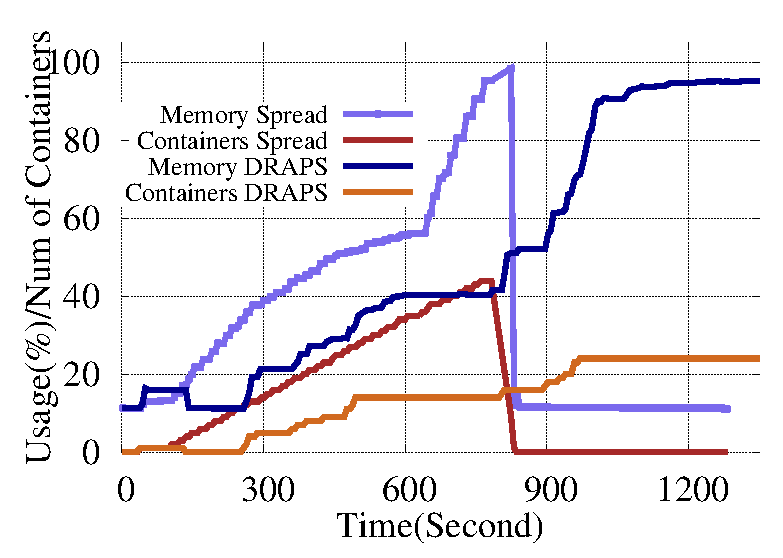
\includegraphics[width=\linewidth]{120workload}
      \caption{Memory usage and container number on worker1}
      \label{fig:120workload} 
      \end{minipage} %
      %%%%%%%%%%%%%%%%%%%%%%%%%%%%%%%%
      \begin{minipage}[t]{0.48\linewidth}
\centering
      \includegraphics[width=\linewidth]{iowait}
      \caption{Value of I/O Wait on worker1}
      \label{fig:iowait}
      \end{minipage} %
%\caption{Resource demonds under different workloads on four services, MySQL, Tomcat, YUM, PI.}
\end{figure}
%\end{comment}
